\chapter{Friction estimation method}

This chapter will describe the chosen method that has been used to estimate the tire/road friction. Different approaches are weighted where a great deal of effort has been put on dealing with the fact that the method should work well in a practical manner, rather than during simulations.

\section{Approach}
The main idea for how to estimate friction is the following. Two models describing the vehicle forces and the tire forces are used. The next step is to make sure that all parameters for the vehicle model is known and that all parameters for the tire model except the tire/road friction coefficient is known. Finally, by fitting the tire model to the vehicle model with recursive least square fitting, using the tire/road friction coefficient as fitting parameter, the tire/road friction coefficient can be estimated. This is true because the forces generated by the tires should be equal to the total force acting on the vehicle.

The first step of the method include calculations of the forces acting on the vehicle by using a vehicle model. This is for example done by using measured and calculated parameters such as wheel speed, yaw rate and acceleration but it can be done in other ways as well. Two different models that describes the vehicle forces will be presented in this work. 

The second step is to calculate the forces generated by the tires through a tire model. Such a model often depend on the tire stiffness, the tires slip ratio, the normal force acting on the tire and the road friction coefficient. Several tire models exists today and in this work three of them will examined more closely. It's in combination with the tire force calculations that the recursive least squares fitting is executed as well. This will also be explained in more detail. 

\subsection{Practical restrictions and problems}
The idea presented above might sound like a very simple solution but there are several problems that have to be considered. The most important aspect that has to be taken into account is the fact that the friction estimation model has to work in a real car handled in actual driving situations. In a theoretical world, where a vehicle and a tire model is fed unbiased data, the friction coefficient can be obtained with good certainty and quite fast. Unfortunately, in the practical world, the data fed to the models are far from optimal. Things like measurement noise and approximative calculations corrupts the results. Several more complex driving situations are also hard to model correctly. This can for example be excessive wheel spin, aggressive cornering or speeds close to zero.

The true dynamics of both a vehicle and a tire is very complex and therefore also difficult to describe accurately with a model. At the same time, a model that is to be used has to be simple enough so that calculations are possible on an micro control unit with limited computational power. Even though many simplified models are shown to be accurate enough to reflect reality in most driving situations, there are times when a simplified model inaccurately describes the detailed dynamics of a vehicle or a tire. 

There are also numerous models that use parameters which are hard to measure or approximate well in reality. Some of these parameters include the lateral velocity and slip angle. It is therefore desired to have a model that doesn't rely on these parameters. There are also car specific parameters, some which change between driving sequences, that can have a large impact on the modeled results. A few of these parameters include the mass of the vehicle, wheel radius, wind drag coefficient, lengths from center of gravity to the rear and front axle and the center of gravity height. When using simulations, the exact value of these parameters can be known, but in a real environment they either have to be static, approximated or neglected in computations.

\subsection{FXD}
The problem stated in this work is to estimate the tire/road friction for a car using an FXD. This results in a number of conditions that have to be thought of and applied throughout the research. First of all, cars with an FXD installed are solely front wheel driven, meaning that there are no positive longitudinal forces acting on the rear wheels. The velocity of the rear wheels can therefore in most cases be used as a good approximation of the vehicles reference speed. Through the same reasoning, the longitudinal acceleration of the car can be derived from the derivative of the rear wheel velocities. There is also no steering done by the rear wheels.

Another aspect that has to be considered is that the FXD is an active limited slip differential, which means that the torque applied to the two driving shafts can differ in certain situations, unlike a car equipped with a standard open differential.

\subsection{Related work}
There have been quite extensive amount of research within this field of study and many different model proposals related to friction estimation during the last decades. The outcome of these researches usually show promising results, where the proposed solution works well during simulations and/or testing. Related work has provided a lot of information and help to this work, especially when it comes to getting a general understanding of the problem and its difficulties. But due to the fact that many results are based on theoretical simulations, a lot of information could be of little use or in some cases even be misleading.

\subsection{Conclusion}
All in all it is a great challenge to estimate the tire/road friction coefficient. \todo{Make sure this is true.} The approach, all of the problems mentioned and how they were taken care of will be explained in greater detail later on in the report.


\section{Vehicle forces}
There are several forces acting on a vehicle. The largest forces are generated between the tires and the ground because the tires are the only parts of a car that have any physical contact with the surrounding world. While accelerating and braking longitudinal forces will arise and while cornering lateral forces will arise. The tires are responsible for all the forces that actually control the vehicle which makes them very important for good handling but also makes them hard to model. Beside these major forces there are also forces such as wind drag and rolling resistance acting on the vehicle.

The trick is to calculate all the forces into one total force that can be compared to the total force generated by the tires.
\subsection{Vehicle force calculated with longitudinal acceleration}
The simplest way of representing the force acting on the vehicle while accelerating is to use the acceleration and the mass of the car and apply Newtons second law of motion:
\begin{equation}
	F = m \cdot a
\end{equation}
\subsubsection{Estimating the longitudinal acceleration}
For this method to be accurate an accurate estimation of the longitudinal acceleration is needed. Some cars have accelerometers installed for longitudinal measurements which makes it straight forward to calculate the force. If one of those aren't available the acceleration has to be calculated instead. This can be done by derivation of the vehicles speed. The speed of the vehicle can be obtained by measuring the speeds of the undriven wheels. For a FWD car this would be the rear wheels. To make the calculation more accurate the average speed of the two rear wheels is calculated before the derivation is done.
\begin{equation}
a_{x} = \frac{d}{dt}(\frac{w_{rl}+w_{rr}}{2})
\end{equation}

\subsubsection{Estimating the total vehicle force}
This measured or derived acceleration is merely the resulting net force acting on the vehicle mass. The total amount of force that is generated from the tires and up to the body has to include the rest of the forces acting on the vehicle. The resulting force that is generated therefore becomes: \todo{this formula might be altered}
\begin{equation}
F_{vehicle} = m \cdot a + F_{steering loss} + F_{wind drag} + F_{rolling resistance}
\end{equation}

\subsubsection{Complications}
One major issue with this method is to obtain a proper value for the longitudinal acceleration. Measuring it with an accelerometer works good as long as the vehicle is driven on a flat road. When driving uphill or downhill the value from the accelerometer will be biased since the earths gravity will affect it. To correct this the angle of the vehicle relative the earths horizontal plane would be needed but this is hard to measure or estimate. \todo{is it really?}

\todo{continue}

A problematic situation for this method occurs when the vehicle is accelerating on a gradient road. During an uphill acceleration, the actual forces acting on the car will be higher than the force calculated from the formula. When driving downhill, the force will be lower.


\subsection{Longitudinal force from engine torque}

Another way of calculating the longitudinal force of a vehicle is to derive the actual torque that is applied to the shafts connected to the driving wheels. The advantage of using the engine torque, instead of the acceleration of the vehicle, is its independence of the roads gradient and losses such wind drag and steering losses. The torque that is applied to the shafts will be directly proportional to the actual force generated to the wheels, regardless of how the gravitational pull and other losses are acting. 

This method include some negative aspects that have to be thought of. It is unfortunately very uncommon for a commercially available vehicle today to have a torque sensor mounted, which means that the torque has to be obtained with other parameters. The torque applied to driving shaft is simply the torque generated from the engine multiplied by the current gear ratio. 
\begin{equation}
\label{eq:tshaft}
T_{shafts} = T_{engine}*Gear Ratio
\end{equation}
Where the gear ratio is the speed exchange from the engine shaft to the wheel shaft.
\begin{equation}
\label{eq:GR}
Gear Ratio = \frac{RPM_{engine}}{RPM_{drivenwheel}}
\end{equation}
The engine torque, engine speed and the wheel speeds are all parameters commonly found on the CAN bus of a newer car. Important to notice is that these calculations do not consider any losses from the engine out to the wheels.

The torque will be split evenly between the two shafts, assuming an open differential, i.e. when the FXD is inactive. By combining equations $ \ref{eq:GR} $ and $ \ref{eq:tshaft} $, it is also seen that the power generated by the engine and the power outputted to the shafts are equal.
\begin{equation}
	P = T_{shafts}*RPM_{wheel} = T_{engine}*RPM_{engine}
\end{equation}

\subsubsection{Transfer losses}
There are losses. We found Magic Formula 2.0.



There are several factors that affect how much of the engine torque that actually generates a driving force between the road and the tire. There are losses in form of friction within the driveline, and also rotating masses within the vehicle that have moment of inertias. 

The frictional losses are very dependant on the design of the engine, driveline, and transmisson. This means that the losses will differ between vehicle models and therefore there are no good model that can represent such losses accurately. It is however known that there are larger losses when the gear ratio transmission is larger. The losses due to higher gear ratio can be described as
\begin{equation}
	Loss\% = \frac{1}{1 + factor(0.0025?)*gearratio^2}
\end{equation}

Each wheel connected to a driven shaft has its own moment of inertia which will be accelerated if enough torque is applied. The amount of torque needed to accelerate the wheel depends on its moment of inertia and the angular acceleration
\begin{equation}
	T = a \cdot I
\end{equation}
Where the moment of inertia is the sum of its integrated mass multiplied by its radii squared. 
\begin{equation}
	I = \int r^2 \cdot dm
\end{equation}
Assuming that a wheel has a shape of a solid cylinder with equal amount of density throughout, the moment of inertia for a wheel can be described as
\begin{equation}
	I = \dfrac{r^2 \cdot m}{2} 
\end{equation}
In the same manner, this applies for the actual shaft as well. 

By subtracting this torque from the shaft, the final torque which generates force between the tire and ground is obtained.
\begin{equation}
	T_{resulting} = T_{shaft} - T_{wheel acc}
\end{equation}
Thereafter the force, in $ N $, can be obtained by dividing the torque, in $ Nm $, by the radii of the wheel
\begin{equation}
	F_{tire} = \frac{T_{resulting}}{r_{wheel}}
\end{equation}
A restriction that has to be thought of is that the amount of force that can be generated between the tire and the road is limited by the tire/road friction and the normal, $ \mu \cdot F_{z} $. Any additional torque applied to the shaft will add to $ T_{wheelacc} $ and merely serve as unwanted acceleration of the wheel, i.e. spinning.


\section{Tire forces}
To calculate the tire force properly the slip angle is needed. 

The characteristics of a tire is very complex, which makes the actual forces generated to the vehicle  difficult to obtain. The main dynamic parameters of existing longitudinal tire force models include the slip ratio, normal force, and the tire/road friction coefficient, $ \mu $:
\begin{equation}
F_{tire} = f(\kappa, Fz, \mu, C_{x})
\end{equation}
The slip ratio is calculated from the wheels difference in angular and forward velocity as seen in equation $ \ref{eq:longslip} $, the normal force from the weigh of the vehicle and the changing weight distribution derived (IN PREVIOUS CHAPTER), and the tire stiffness as explained  in (IN PREVIOUS CHAPTER). Thereafter, the only dynamic parameter of the tire force equation becomes the friction coefficient. By choosing the correct $ \mu $, the force from the tire model will equal the force from the vehicle model. This calculation is done in a feedback manner, meaning that the tire force depends on the friction coefficient derived in the previous iteration.

\begin{figure}[h]
	\centering
	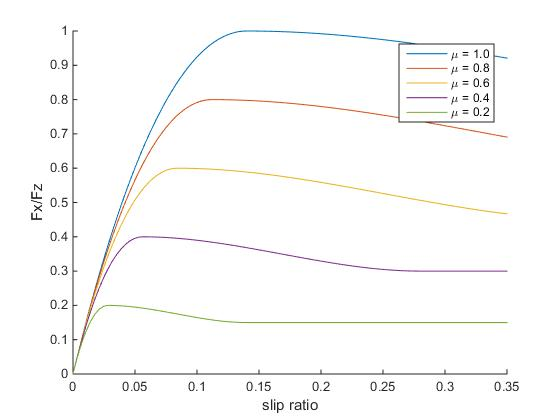
\includegraphics[width=0.8\textwidth]{Pictures/force_per_slip_different_mue}
	\caption {Normalized tire model force per slip ratio for different mue.}
	\label{force/slip}
\end{figure}


\subsection{Tire stiffness}

Tires stiffness mentioned earlier. Problem is that different tires have different stiffness, but the driver shouldn't have to say what kind of tires that are used. Should be detected!

The tire stiffness is obtained by deriving how much force the tires generates per slip for low slip values, e.i. in the linear region. Unfortunately, a tire characteristics is further complex, and cannot be explained by this one parameter alone. Two different tires can have the same tire stiffness, but different characteristics for larger slip ratio values. An example of this can be seen in Figure [twi tires].

The tire stiffness will also be different for different road surfaces. Even in the linear region, the same amount fo slip will generate more force on asphalt than on snow or ice. 

\subsection{Slip ratio}

Important to get accurate slip ratio. Different tire size = no good!

As seen in most slip/force figures, the maximum force will be generated at a specific slip and thereafter decrease as the slip increases. If the chosen tire model does not explain this peak in force correctly, the force from the tire model will be very difficult to match the vehicle force acting. 

The value of the slip ratio is rather small (maximum force is generally obtained at a slip ratio $ \geq 12 \% $), which means that variances in the slip ratio calculations will have a large impact. The four wheel speeds that are obtained from the vehicles CAN usually include quite a lot of noise [Figure blah, part 1]. The signals will after filtering still have an oscillating attribute due to the characteristics of the wheel speed sensor and its design [Figure blah, part 2]. When the oscillations from the front and its respective rear wheel are not synchronized, the variation of the calculated slip ratio will be even larger.

Another concrete problem that arises when calculating the slip ratio, is that the radius for each wheel on a vehicle can be different, e.g. when the air pressure of a tire has changed slightly. The wheel speed obtained from the CAN will in this case be wrong, leading to a offset in the slip ratio.

\subsection{Normal force}

Longitudinal/lateral force generated from tire depends on the normal force on that tire. Maximum tire force
\begin{equation}
	F \leq F_{z*\mu}
\end{equation}

The force generated by a tire is linearly proportional to the normal force on the tire. 


\section{Signal processing}

Signals are noisy on CAN!



\subsection{Filters}

Signals need to be filtered. Low-pass, high-pass. High damping for Cx etc..


\subsubsection{Timing of signals}

Due to filtering (multiple filtering(acc)), signals delayed, have to be timed.

Different signals have different noise, and therefore should be filtered differently, this leads to signals being delayed against each other. 

\subsection{Static parameter impact}

Massa, radie på hjulen, CGO height, osv..

\section{Other methods}

\subsection{Slip-slope friction model}

One friction model that is frequently used and referred to in research papers is the so called slip-slope friction model. The models general idea is that the maximum tire/road friction available can be decided due to its dependency on the slope from the slip-force curve in the linear region. This slip-force curve has the same characteristics as the slip-friction coefficient curve seen in Figure \ref{fric_slip}. 
\begin{equation}
\dfrac{F_{x}}{F_{z}} = k \cdot \kappa
\end{equation}
Where $ F_{x} $ and $ F_{z} $ is the estimated longitudinal and normal force acting on a tire depending on input values. The slip-slope can be estimated with for example recursive least square fitting.
